\documentclass[a4paper,11pt]{article}
\usepackage{a4wide,amsmath,ngerman,url,graphicx}
\usepackage[utf8]{inputenc}
\parskip4pt
\parindent0pt

\newcommand{\br}[1]{\left(#1\right)}
\newcommand{\erf}{\mathrm{erf}}
\newcommand{\m}{\cdot}

\title{Analyse der Coronastatistiken. Teil 1} 
\author{Hans-Gert Gräbe, Leipzig}
\date{Version vom 13. April 2020, mit kleinen Korrekturen vom 31. Mai 2020}

\begin{document}
\maketitle

Dieser Text bezieht sich auf eine erste Version\footnote{Nachtrag: Es wurden
  bewusst nur kleine Korrekturen an dieser erste Version angebracht, um die
  spezifische Situation einer unklaren Zukunft zu erhalten, auf die mit einer
  ersten Parameterschätzung Ende März 2020 und einem Update am 13.04.2020
  reagiert wurde. Der Wert der Schätzungen auf realen Daten wird im Teil 3
  diskutiert.} der im Verzeichnis
\url{http://leipzig-data.de/demo/Corona-20/Code} verfügbaren Materialien.

\section{Datenbasis}

Als Datenbasis werden die von der Johns Hopkins Universität (JHU) als
Excel-Datei veröffentlichten Daten\footnote{Siehe deren github-Projekt
  \url{https://github.com/CSSEGISandData/COVID-19}.} zur Entwicklung der
weltweit registrierten Covid-19-Fälle verwendet. Die Statistik listet pro Land
und Tag die kumulierte Zahl der positiv Getesteten\footnote{Nachtrag: statt
  „Infizierte“, wie in der ersten Auf"|lage noch geschrieben.  Dies ist hier
  konsequent an allen Stellen ersetzt.}, der Genesenen und der Todesfälle auf.

Die Statistiken sind natürlich zu hinterfragen, da sich jedem Physiker die
Haare sträuben würden, wenn die Debatte auf die messmethodische Grundlage
dieser Datenerhebungen, also die Einheitlichkeit des Modells, zu sprechen
kommt.  Dennoch gibt es wohl derzeit nichts Besseres. Auch die Rolle der
privaten (!)  JHU und deren enge Verflechtung mit dem „Datenadel“ aus dem
Silicon Valley kann hinterfragt werden, siehe dazu (Rügemer 2020).  Spannend
auf der anderen Seite, dass es genau dieser „Datenadel“ ist, der solche Daten
zusammenträgt und der Allgemeinheit -- im Gegensatz etwa zu der im deutschen
Sprachraum viel zitierten \url{https://statista.com} oder gar der WHO -- in
einem maschinenlesbaren Format ohne Bezahlschranken zur Verfügung stellt.

Eine solche kritische Würdigung muss diesem Text vorangestellt werden, um die
folgenden Rechnungen ins rechte Licht zu rücken, denn sie sind nicht als
Beitrag zur Corona-Debatte selbst gedacht, wie dies in den ersten Tagen
mehrfach falsch verstanden wurde, sondern soll die Möglichkeiten aufzeigen,
die fortgeschrittene Oberstufenschülerinnen und -schüler heute zu einer
eigenen Analyse von Daten haben.  Der komplexe Gegenstand „CAS in der Schule“
ist in meinem Buch (Gräbe 2018) genauer dargestellt. 

\section{Installation} 

Zunächst muss das git Repo der JHU lokal geklont und der Pfad im Skript
\texttt{extractData.pl} eingetragen werden.  Die Daten werden für ausgewählte
Länder mit diesem Perl-Skript für die weitere Verarbeitung aufbereitet und in
einer Datei \texttt{BasicData.txt}\footnote{Nachtrag: Inzwischen in
  \texttt{BasicData-Maxima.txt} umbenannt, da die Möglichkeiten des CAS
  \emph{Maxima} zum nichtlinearen Fitting beschränkt sind und gelegentlich
  meinen Laptop insgesamt zum Stillstand bringen.} gespeichert, um dann mit
dem freien CAS \emph{Maxima} weiterverarbeitet zu werden.

\section{Datentransformation}

In der Datei \texttt{BasicData.txt} sind die Daten für jedes der ausgewählten
Länder in einem Array mit drei Einträgen (infected, recovered, dead)
gespeichert, die im Maxima-Skript \texttt{skript.m}\footnote{Dies ist eine
  reine Textdatei mit Code-Schnipseln, die nicht für den Batchbetrieb
  konzipiert ist.} in einer Funktion \texttt{getland(Land)}\footnote{Nachtrag:
  Diese Funktion wurde inzwischen umgeschrieben und gibt nun eine größere
  Menge von Datenreihen zurück, die für verschiedene Auswertungszwecke aus den
  drei originalen Datenreihen der JHU gewonnen werden.} zunächst einmal zu
Paaren $(t,y_t)$ ergänzt werden, wobei $t$ für den Tag des Jahres 2020
($1=01.01.2020$, \textbf{Tag 100 ist also Donnerstag, der 9. April}) und $y_t$
für die Zahl der Fälle aus dem jeweiligen Record stehen.

\section{Fitting}

Alle Grafiken zu Prognosen der Daten, die ich bisher gesehen habe, gehen von
einer „Glockenkurve“ aus.  Das kann natürlich nur die Entwicklung der Zuwächse
pro Tag abbilden, die aus den kumulierten Daten zunächst als $d_t=y_t-y_{t-1}$
extrahiert werden müssen. Dies geschieht mit der im Skript definierten
Maxima-Funktion \texttt{Delta}\footnote{\texttt{reverse(rest(reverse(l)))}
  entfernt das letzte Element der Liste, \texttt{append([0],...)} fügt vorn
  eine $0$ an, womit eine Liste $l_1$ entsteht, in der alle Einträge um eine
  Position nach rechts verschoben sind. $l-l_1$ berechnet die Differenz der
  Listen, was in Maxima (und anderen CAS) als Subtraktion der entsprechenden
  Vektoren implementiert ist.}.

Zur Abschätzung des Verlaufs längs einer Glockenkurve wird üblicherweise die
Statistikfunktion $C\m\exp\br{-\br{\frac{t-m}{s}}^2}$ verwendet, die ich als
Kurvenschar $f(t)=\exp\br{c-\br{\frac{t-m}{s}}^2}$ zur Parameterschätzung auf
die Daten $(t,d_t)$ ansetze.  Die (kumulierten) Originaldaten $(t,y_t)$
sollten dann auf die Funktion
\begin{align*}
  h(x)&=\int_0^x{\exp\br{c-\br{\frac{t-m}{s}}^2}}\,dt\\ &=\exp(c)\m s\m
  \int_{-\frac{m}{s}}^{\frac{x-m}{s}}{\exp\br{-u^2}}\,du\\ &=\frac12 \sqrt{\pi}\m
  \exp(c)\m s\m \br{\erf\br{\frac{x-m}{s}}+ \erf\br{\frac{m}{s}}}
\end{align*}
matchen, wobei $\erf(x)$ für die Fehlerfunktion steht und im zweiten Schritt
die Variablensubstitution $u=\frac{x-m}{s}$ mit $du=s\m dt$ erfolgte.

Nun sind die Parameter $(c,s,m)$ dieser Kurvenschar so zu fitten, dass die
ermittelte Kurve besonders gut auf die Daten passt.  In \emph{Maxima} kann
dazu das Paket \emph{lsquares} verwendet werden.  

Wir hätten natürlich auch versuchen können, die Originaldaten auf die Schar
$h(t)$ zu fitten, aber Fitting auf nicht polynomialen Kurvenscharen ist eine
schwierige und numerisch wenig stabile Angelegenheit, bei der Maxima schnell
an seine Grenzen kommt (und die Ergebnisse anderer CAS sehr genau zu
analysieren sind, da die Fitting-Ergebnisse stark von Startwerten der dabei
eingesetzten Verfahren abhängen).

\emph{Maxima} kommt auch beim Fitting der Schar $f(t)$ zu keinem Ergebnis.
Einen einfacheren, nämlich quadratischen Zusammenhang
$g(t)=c-\br{\frac{t-m}{s}}^2$ erhält man, wenn man zu Paaren $(t,\log(d_t))$
übergeht.  Damit lassen sich dann die Fittingparameter weitgehend stabil
berechnen. Dafür müssen aber vorher Datenpunkte aussortiert werden, wo $d_t=0$
ist.

Generell kann es sinnvoll sein, für ein gutes Fitting Datenpunkte unterhalb
einer Schwelle auszusortieren. Eine solche Schwelle $S$ ist als weiterer
Parameter im Skript in der Funktion
\texttt{FittingDelta(G,S)}\footnote{Nachtrag: Mit der Änderung von
  \texttt{getData(Land)} wurde auch diese Funktion verändert, da die
  Datenreihen $(t,d_t)$ nun bereits in \texttt{getData(Land)} berechnet
  werden.} vorgesehen. Für die meisten Datensätze ist die Schwelle 50 eine
gute Wahl. $G$ ist die Liste $(t,y_t)$ der zu fittenden Datenpunkte.

Details sind im Skript \texttt{skript.m} zu finden.

\section{Ergebnisse}

Die Rechnungen werden für jedes der Länder nun wie folgt ausgeführt:
\begin{enumerate}
\item Fasse mit \texttt{l:getData(Land)} die drei Datensätze für das Land als
  Tripel von Listen $(t,y_t)$ zusammen.
\item Berechne für jeden der drei Datensätze mit
  \texttt{getFittingFunctions(l,S)} das Fitting auf $(t,\log(d_t))$ gegen die
  Funktion $g(t)$ und verwende die berechneten drei Fittings, um Funktionen
  $h_1(t)$ (für positiv getestet), $h_2(t)$ (für genesen) und $h_3(t)$ (für
  verstorben) zu schätzen.
\item Erzeuge daraus einen Plot, welcher die Datenpunkte und die drei Kurven
  in verschiedenen Farben (rot für positiv getestet, grün für genesen, blau
  für verstorben) ausgibt.
\end{enumerate}
Bei erfolgreichem Fitting ist eine gute Übereinstimmung der jeweiligen
Kurve\footnote{Für $x=\frac{m}{s}\approx 10$ kann $\erf(x)=1$ gesetzt werden.
Ist dieser Wert im Fitting deutlich anders, ist das Fitting unbrauchbar.}
\begin{gather*}
  h(t)=A\br{\erf\br{B(t-m)}+1}
\end{gather*}
mit den Datenpunkten zu verzeichnen.  Die berechneten Parameter haben folgende
Bedeutung:
\begin{itemize}
\item $m$ -- Tag, an dem die Spitze in den Inkrementdaten erreicht ist.
\item $B=\frac{1}{s}$ -- $\sigma=\frac{s}{\sqrt{2}}$ ist die
  Standardabweichung.
\item $2A$ -- Zahl der am Ende insgesamt betroffenen Personen. 
\end{itemize}

Auf der Basis der Daten vom 13.04.2020 lassen sich folgende Szenarien (!) für
die Länder Deutschland, Italien, Spanien, Österreich und Schweden erstellen,
siehe auch die Abbildungen.

Alles begann in der chinesischen Provinz Hubei (mit 58.5 Mio. Einwohnern hat
sie eine mit Italien vergleichbare Einwohnerzahl).  Auch die dortige
Entwicklung ist dargestellt\footnote{Maxima hängt sich bei der Berechnung
  dieses Fittings allerdings schnell auf.}.

\begin{center}
  \begin{tabular}{|l|r|r|r|}\hline
    & \multicolumn{1}{|c|}{$m$} & \multicolumn{1}{|c|}{$s$}
    & \multicolumn{1}{|c|}{$A$} \\\hline
    \multicolumn{4}{|c|}{\bf Deutschland}\\\hline
    positiv getestet   & 91.94 & 13.51 &  68896\\
    genesen  & 97.01 &  8.58 &  32967\\
    verstorben       &103.11 & 14.80 &   3241\\\hline
    \multicolumn{4}{|c|}{\bf Italien}\\\hline
    positiv getestet   & 88.34 & 16.30 &  87225\\
    genesen  &101.35 & 21.97 &  31380\\
    verstorben       & 90.31 & 16.07 &  11520\\\hline
    \multicolumn{4}{|c|}{\bf Spanien}\\\hline
    positiv getestet   & 91.11 & 12.32 &  90706\\
    genesen  &101.77 & 15.78 &  54984\\
    verstorben       & 93.33 & 11.88 &   9611\\\hline
    \multicolumn{4}{|c|}{\bf Österreich}\\\hline
    positiv getestet   & 88.55 & 12.09 &   6651\\
    genesen  &100.02 & 10.68 &   5319\\
    verstorben       & 98.62 & 17.12 &    294\\\hline
    \multicolumn{4}{|c|}{\bf Schweden}\\\hline
    positiv getestet   &101.08 & 20.75 &   8870\\
    genesen  &112.73 & 20.12 &   4402\\
    verstorben       & 95.36 &  9.09 &    459\\\hline
    \multicolumn{4}{|c|}{\bf China, Provinz Hubei}\\\hline
    positiv getestet   & 41.45 & 13.12 &  26139\\
    genesen  & \multicolumn{3}{|c|}{bad fitting}\\
    verstorben       & 46.74 & 15.72 &   1759\\\hline
  \end{tabular}
\end{center}
Natürlich müsste am Ende die Zahl der Infizierten mit der Summe der Zahlen der
Genesenen und der Verstorbenen übereinstimmen.  Die Schätzungen sind von einer
solchen Invarianzforderung weit entfernt, was ein Licht auf die prognostische
Qualität der Schätzungen für die weitere Zukunft (drei bis vier Wochen, also
30 Tage) wirft.  Weitere Ergebnisse zeigen, dass selbst einem ohne
Fehlermeldung zurückgegebenen Fitting nicht zu trauen ist und die Güte des
Fittings genauer analysiert werden muss.  Die Ergebnisse für die Provinz Hubei
legen nahe, dass das verwendete Datenmodell für die Schätzung generell wenig
geeignet ist, da die Zahl der Infektionen selbst im Nachgang zu klein
geschätzt wird und für die Zahl der Genesenen kein brauchbares Fitting
gefunden wird, obwohl sich die Zahlen in Bereichen bewegen, wie sie auch für
europäische Länder charakteristisch sind.

\section{Literatur}

\begin{itemize}
\item Hans-Gert Gräbe. Computeralgebra im Abitur. Reihe „Eagle Starthilfe“.
  Eagle Verlag, Leipzig 2018.  Siehe
  \url{https://hg-graebe.de/CAimAbitur/index.html}.
\item Maxima. \url{http://maxima.sourceforge.net/de/}. Das CAS ist in
  Linux-Distributionen über den Paketmanager leicht zu installieren.
\item Werner Rügemer. „Die USA haben das sicherste Gesundheitssystem der Welt“
  – Die Johns Hopkins University und das globale Pandemien-Management.
  01.04.2020.\\ \url{https://www.nachdenkseiten.de/?p=59825}
\end{itemize}

\section{Grafiken}

\begin{center}
  \begin{minipage}{.48\textwidth}\centering
  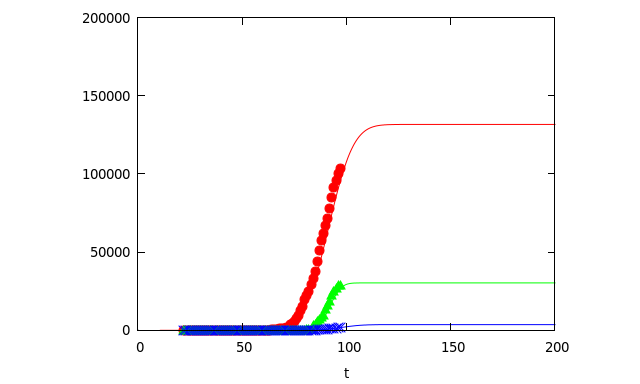
\includegraphics[width=\textwidth]{Germany.png}\\[1em]
  {Szenario für Deutschland\\ (82.9 Mio. Einwohner)}
  \end{minipage}\hfill
  \begin{minipage}{.48\textwidth}\centering
  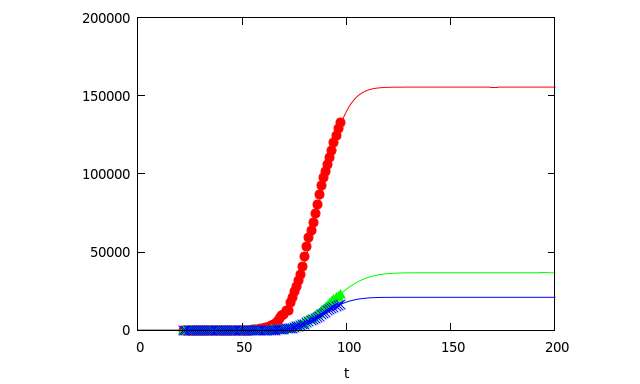
\includegraphics[width=\textwidth]{Italy.png}\\[1em]
  {Szenario für Italien\\ (60.4 Mio. Einwohner)}
  \end{minipage}
  
  \begin{minipage}{.48\textwidth}\centering
  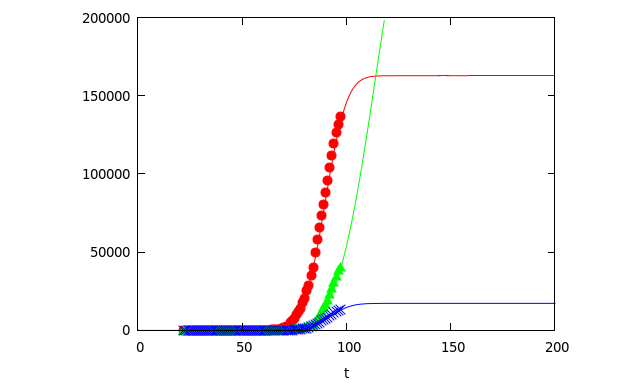
\includegraphics[width=.8\textwidth]{Spain.png}\\[1em]
  {Szenario für Spanien\\ (46.7 Mio. Einwohner)}
  \end{minipage}\hfill
  \begin{minipage}{.48\textwidth}\centering
  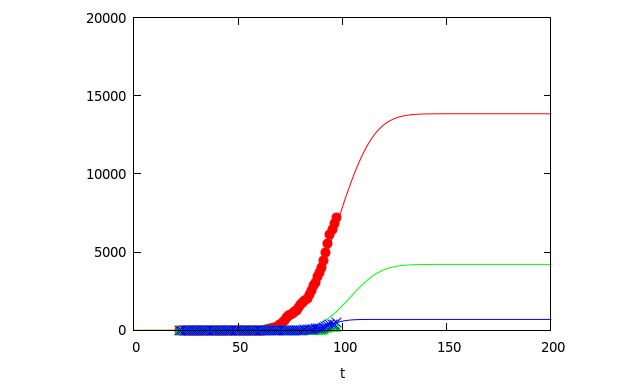
\includegraphics[width=.8\textwidth]{Sweden.png}\\[1em]
  {Szenario für Schweden\\ (66.4 Mio. Einwohner)}
  \end{minipage}
  
  \begin{minipage}{.48\textwidth}\centering    
  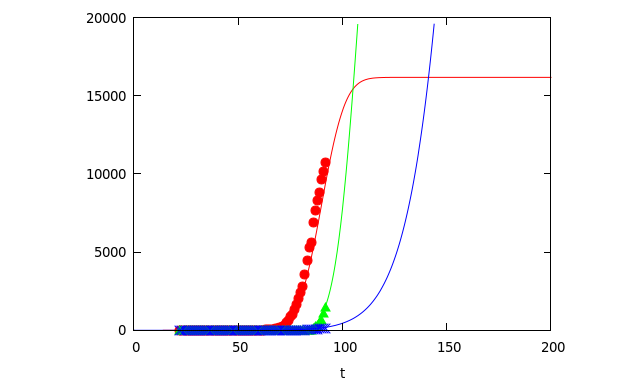
\includegraphics[width=.8\textwidth]{Austria.png}\\[1em]
  {Szenario für Österreich\\ (8.85 Mio. Einwohner)}
  \end{minipage}\hfill
  \begin{minipage}{.48\textwidth}\centering                  
  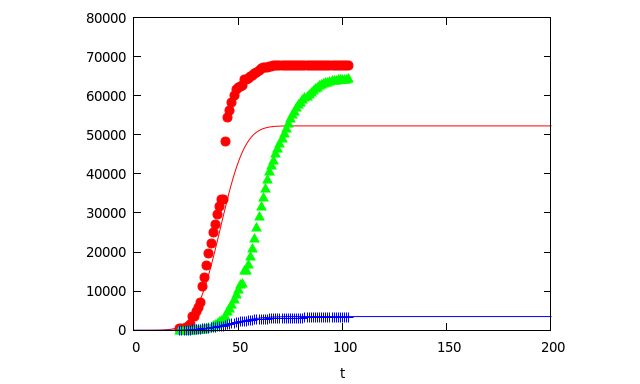
\includegraphics[width=.8\textwidth]{Hubei.png}\\[1em]
  {Szenario für China, Provinz Hubei\\ (58.5 Mio. Einwohner)}
  \end{minipage}
\end{center}


\end{document}
